\documentclass[conference]{IEEEtran}

\usepackage[T1]{fontenc}
\usepackage{booktabs}
\usepackage{graphicx}
\usepackage{microtype}
\usepackage{xspace}
\usepackage{url}

\newcommand{\system}{\textsc{Tarsus}\xspace}
\newcommand{\putop}{\textsc{put}\xspace}
\newcommand{\readop}{\textsc{read}\xspace}
\newcommand{\getop}{\textsc{get}\xspace}

% ICDCS uses double-blind review. Change to \anonymousfalse only for an
% internal or camera-ready copy.
\newif\ifanonymous
\anonymoustrue

\begin{document}

\title{Tarsus: A Tuple Space for Content-Addressed Distributed Storage}

\ifanonymous
\author{\IEEEauthorblockN{Anonymous Authors}}
\else
\author{
\IEEEauthorblockN{Nick Tagliamonte, Justin Y. Shi, and Garrett Stoll}
\IEEEauthorblockA{Temple University\\
Philadelphia, Pennsylvania, USA\\
\{tug35742,shi,tuv14706\}@temple.edu}}
\fi

\maketitle

\begin{abstract}
Content-addressed storage retrieves immutable data efficiently once its
identifier is known, but distributed applications must also discover work by
its properties and assign that work without a central queue. We present
\system, a peer-to-peer storage system with an integrated, Linda-style tuple
space. Applications publish, observe, and exclusively consume tuples through
\putop, \readop, and \getop, while bulk content remains in a separately routed
and hash-verified data plane. Exact tuple names have deterministic owners that
serialize mutations. Associative queries use hash-sharded Prefix Hash Trees
and Bloom summaries to find candidate names, then contact exact owners for an
authoritative result. Durable request results and epoch fences extend
exclusive consumption across bounded crash handoff without claiming consensus
during arbitrary partitions.

We evaluate 10,500 query trials in fresh clusters of up to 90 peers and
catalogs of 10,000 tuples. At 90 peers, exact reads have a 0.77-ms median.
Bloom pruning improves a selective substring query by 2.69$\times$ and fetches
3.18$\times$ fewer index nodes, but hurts broad queries, exposing when pruning
is worthwhile. Four index shards improve population throughput by
3.10$\times$ over one shard, while further sharding raises query fanout. Every
associative trial returned an owner-verified match, including 600 trials in the
64-shard cell despite partial shard responses. A 100-peer failure case retains
access to an 8-MiB object after one of seven providers stops and restores the
replica target in 51.3 s. These results characterize both the usefulness and
the current limits of tuple coordination over a content-addressed substrate.
\end{abstract}

\begin{IEEEkeywords}
tuple space, distributed storage, associative matching, content addressing,
distributed hash table, peer-to-peer systems
\end{IEEEkeywords}

\section{Introduction}

Content addressing gives distributed storage a stable answer to ``which bytes
are requested?'' A client supplies a digest-derived identifier, a routing
system locates providers, and the client verifies the returned bytes. This is
an effective data model for immutable objects, but it assumes the client
already knows the identifier. Many distributed applications begin with a
different question: is there an unclaimed task for this data set, has any
worker produced a result with these properties, or which available peer can
host another replica?

These are coordination questions. Deployments commonly answer them with a
central database, message broker, or scheduler layered over decentralized
storage. The additional service becomes both an authority and an availability
dependency: replicated bytes can remain accessible while applications can no
longer discover or exclusively claim the work those bytes represent.

Tuple spaces provide a compact alternative. Producers place tuples into a
shared associative space; consumers inspect or remove matching tuples without
knowing producer identities or locations. The interface decouples participants
in time and space and naturally expresses work queues, result discovery, and
resource advertisements. Linda introduced the best-known tuple-space model
\cite{Gelernter1985,CarrieroGelernter1989}; \system uses its coordination style
but is a new implementation and does not embed or depend on Linda.

\system integrates such a tuple space into a content-addressed peer-to-peer
store. A tuple may describe a task and reference immutable content, but the
content bytes do not pass through the tuple space. Exact-name tuple state is
owned and serialized at a deterministic overlay peer. Prefix and substring
queries discover candidate names through distributed indexes; candidates
remain hints until an exact owner verifies and, for \getop, atomically removes
one tuple instance. This separation keeps associative discovery from becoming
a bulk-data broadcast and keeps stale index entries from authorizing duplicate
consumption.

Two terms inherited from the broader project describe how these pieces fit.
An \emph{Active Content Addressable Network} (ACAN) augments immutable content
keys with tuples that participate in discovery, placement, and repair.
\emph{Statistic Multiplexed Communication and Computing} (SMC2) selects among
currently observed peer resources---using availability, connectivity,
round-trip time, storage offers, and optional reputation---rather than binding
an object permanently to its first provider. ACAN and SMC2 are architectural
roles in \system, not new consistency models.

This paper contributes:

\begin{itemize}
  \item a single tuple-space interface for application coordination and active
  storage metadata over a content-addressed data plane;
  \item a query-sensitive design that combines deterministic exact-name
  ownership with hash-sharded Prefix Hash Trees (PHTs), Bloom pruning, and
  authoritative owner verification;
  \item an explicit consistency boundary for non-consuming reads, exclusive
  claims, durable retries, and fenced crash handoff, without overstating those
  mechanisms as partition-tolerant consensus; and
  \item a working Go/libp2p implementation and a 10-cell evaluation that
  quantifies peer and catalog scaling, the index-shard tradeoff, Bloom-filter
  effectiveness, and a bounded provider-failure case.
\end{itemize}

The central contribution is the tuple space and the division of responsibility
around it. Provider records and direct content transfer already exist in IPFS
and related systems; \system does not claim otherwise. Its contribution is to
make associative coordination a first-class operation over the same
peer-to-peer substrate.

\section{Use Case and Requirements}
\label{sec:requirements}

Consider an image-processing workflow spanning several sites. A producer
stores an immutable input and publishes a tuple named
\texttt{task:image:\emph{dataset}:\emph{id}}. Its value contains the content
key and operation parameters. A worker asks for a matching task with
\texttt{task:image:\emph{dataset}:*} and performs a consuming \getop. One
worker obtains the tuple, fetches and verifies the content from a provider,
computes a result, and publishes a result tuple. Observers use \readop to
inspect progress without consuming it.

This small workflow yields five requirements. First, participants must discover
tuples by properties rather than exact identifiers. Second, a consuming claim
must have one authoritative serialization point; discovery alone cannot grant
ownership. Third, a timed-out mutation needs a stable request identity so a
retry does not repeat a committed effect. Fourth, tuple metadata must remain
small while referenced content moves directly between providers and
requesters. Fifth, discovery and storage must continue after ordinary crash
failures when surviving replicas and a connected overlay remain.

These requirements do not imply a POSIX file system. \system currently offers
immutable content objects plus a coordination namespace, not directories,
byte-range writes, rename, access-control lists, or close-to-open cache
semantics. The relevant comparison is therefore to distributed object storage
and coordination services, not to a fully compatible mounted file system.

\section{Interface and Consistency Boundary}
\label{sec:semantics}

\subsection{Tuple Operations}

The tuple space is a multiset: distinct tuple instances may have identical
names and values. Its three basic operations appear in
Table~\ref{tab:operations}. Pattern syntax supports exact names, prefixes,
substrings, and a general expression fallback. \readop and \getop return one
verified match rather than an exhaustive snapshot.

\begin{table}[t]
\caption{Tuple operations. A pattern operation discovers candidate names but
executes against their authoritative exact-name owners.}
\label{tab:operations}
\centering
\begin{tabular}{@{}lll@{}}
\toprule
Operation & State effect & Completion meaning \\
\midrule
\putop$(n,v)$ & add one instance & durable at owner \\
\readop$(p)$ & none & one current match \\
\getop$(p)$ & remove one instance & exclusive claim \\
\bottomrule
\end{tabular}
\end{table}

For an exact name, a Kademlia-key calculation selects the owner. That owner
holds the name's multiset under mutual exclusion. It appends on \putop, copies
the oldest instance on \readop, and selects and removes the oldest instance in
one critical section on \getop. Consequently, while requests resolve to the
same live owner, two successful \getop calls cannot return the same tuple
instance. This is an implementation invariant, not a claim that all tuple
operations form one global serial order.

An associative operation first obtains candidate names and then performs an
exact operation at candidate owners. The index can lag tuple state in either
direction: a recently published tuple might not yet appear, and a deleted name
might remain temporarily. Owner verification converts the latter into extra
work rather than an incorrect match. The former means candidate enumeration is
eventually consistent and can be temporarily incomplete.

\subsection{Durable Retries and Owner Changes}

Each exact-name DHT record contains the multiset, an ownership epoch and writer
identity, a monotonic version, and a bounded map from successful mutation
request IDs to their results. A mutation writes the state transition and its
request result in the same version, rereads the selected DHT value, and only
then acknowledges success. A retry with the same ID returns the recorded
result without applying the transition again.

Ownership uses a lease-bearing epoch fence. After an owner's lease expires, a
successor reads the selected record, preserves both tuple state and retained
retry results, and publishes a higher epoch. DHT validation orders records by
fence before local version, preventing a converged lower-epoch writer from
replacing the successor's state. These mechanisms passed repeated live-DHT
crash-handoff tests, but their scope is deliberately narrower than consensus.
They assume bounded clock error, lease expiry before handoff, and eventual
agreement on the selected DHT value. During arbitrary partitions, \system may
reject or delay work and does not promise linearizable availability across
divergent overlay views.

\begin{table}[t]
\caption{Claim boundary. ``Yes'' is conditional on a connected overlay and
the ownership assumptions in the text.}
\label{tab:claims}
\centering
\begin{tabular}{@{}p{0.47\columnwidth}p{0.42\columnwidth}@{}}
\toprule
Property & Current guarantee \\
\midrule
Altered content accepted & No, absent a hash break \\
Same tuple consumed twice at one owner & No \\
Committed retry repeated in retained window & No \\
Single-owner crash handoff & Yes, under fence assumptions \\
Multi-tuple atomicity & No \\
Availability in arbitrary partitions & No \\
Byzantine metadata agreement & No \\
\bottomrule
\end{tabular}
\end{table}

Content integrity has a separate and simpler boundary. The requester derives
the requested key from the expected digest and returns bytes only if their hash
matches it. A provider may withhold content, and all providers may be
unreachable, but altered bytes cannot be accepted without breaking the hash
assumption. Replica count is an availability policy, not a voting quorum.

\section{Design}
\label{sec:design}

\subsection{One Integrated Tuple Space}

Application tuples, content-provider metadata, storage offers, and repair
coordination use one logical interface. This does not mean that all records
have one physical owner. Exact names distribute across the overlay, and index
shards distribute associative metadata. Integration occurs at the operation
boundary: every record is published and found with the same tuple semantics,
while record type determines how the application interprets its value.

This choice avoids separate discovery systems with incompatible failure and
authorization rules. A worker query and a repair-coordinator query traverse the
same index path and end at authoritative tuple owners. It also exposes a common
failure: if the associative index is stale, both applications can miss recent
records. \system therefore treats the index explicitly as an eventually
consistent acceleration structure rather than as tuple state.

\subsection{Query-Sensitive Routing}

Exact operations need no catalog scan. The tuple name is hashed into the
Kademlia keyspace and the request is sent to its deterministic owner with a
dedicated libp2p stream protocol.

Prefix expressions descend a PHT stored through the DHT
\cite{RamabhadranPHT}. Substring expressions derive n-grams and consult Bloom
summaries on PHT subtrees. A subtree whose summary lacks a required n-gram can
be skipped; surviving names are tested against the original expression, so a
Bloom false positive affects cost but not the returned result. General
expressions retain a catalog matching fallback. This preserves a useful
interface but has linear catalog work in the worst case.

PHT insertion is a read-modify-write operation. Allowing unrelated peers to
modify one index record concurrently caused lost updates in the earlier
prototype. \system instead hashes each full tuple name into one of a fixed
number of PHT shards. A separate mutation key maps each shard to its current
overlay owner, which serializes insertions and deletions within that shard and
publishes versioned PHT nodes. Hashing the full name spreads workloads whose
human-readable names share prefixes such as \texttt{task:}.

Queries read shards in parallel, merge candidate names, and contact exact
owners. Mutation capacity can therefore improve with shard count, but every
indexed query has fixed fanout proportional to the number of shards. The
evaluation shows that this is a real operating tradeoff, not a free scaling
parameter.

\subsection{Metadata and Content Planes}

Content blocks use SHA-256-derived keys. A routing token associates a key with
provider identities and addresses. Retrieval resolves the token, opens direct
streams to providers, and verifies the received bytes. Tuple values may carry
the key and application metadata, but not the bulk content itself.

This design follows a well-established separation. IPFS uses content IDs,
provider records, and direct block exchange; CFS and OceanStore likewise
separate placement and lookup concerns in content-addressed distributed
storage \cite{DabekCFS,KubiatowiczOceanStore,Trautwein2022}. \system's claim is
not that provider/data decoupling is new. The distinctive step is placing
application coordination and active storage metadata in the integrated tuple
space while retaining direct, verified content transfer.

\subsection{ACAN, SMC2, and Repair}

ACAN records make storage state active. Peers advertise available capacity;
provider tuples identify current locations; repair observations remove failed
locations and publish replacements. SMC2 consumes these observations at
operation time. Placement measures peer round-trip times and seeks a configured
mix of near, middle, and far replicas, falling back when a class lacks enough
candidates.

The default replica target is seven: three near, two middle, and two far.
Periodic audits probe providers, elect one reachable repair coordinator,
remove sufficiently observed failures, prefer candidates from missing latency
classes, and then fill any remaining count deficit. Publishing the source
provider before asynchronous copies preserves immediate retrievability. One
coordinator publishes each completed transfer to avoid competing lost-location
updates.

RTT diversity is opportunistic. It can reduce correlated latency failure on a
real multi-region deployment, but containers on one host do not establish
regional independence. Accordingly, our principal campaign evaluates tuple
coordination; the storage failure result is reported as a bounded mechanism
case rather than a geographic-resilience claim.

\section{Implementation}
\label{sec:implementation}

The prototype is written in Go over libp2p. It contains a Kademlia DHT,
content-addressed block storage, routing tokens, direct content fetch, the
native tuple multiset, an exact-owner protocol, PHT nodes implemented through
the DHT value-store interface, hash-sharded index maintenance, Bloom subtree
summaries, fencing and durable retry records, replication and repair streams,
and an HTTP experiment API. The tuple space is implemented in this codebase;
Linda supplies the conceptual lineage only. A legacy adapter remains an
optional compatibility path and is not used by the evaluated configuration.

The query router records query kind, contacted/successful/failed shards, PHT
nodes fetched, branches considered and pruned, index candidates, exact-owner
attempts, verified matches, and end-to-end duration. Mutation coordinators
record local and remote work, failures, per-shard activity, authority changes,
and service time. The experiment endpoint attaches these counters to the
specific request so unrelated background repair advertisements are not counted
as workload insertion.

Tuple requests, streams, and records are bounded and deadline controlled.
Exact-name records currently have a 1-MiB limit, and retry results use a
bounded retention window. The campaign's bulk-insertion endpoint retries only
recognized prepublication index-route failures. It never retries an ambiguous
tuple-owner failure because a lost acknowledgement could follow a committed
\putop; in that path the caller must reuse the request ID.

\section{Evaluation}
\label{sec:evaluation}

Our experiments ask four questions:

\begin{enumerate}
  \item How do peer count and catalog size affect exact and associative query
  latency?
  \item What mutation-throughput/query-fanout tradeoff follows from index
  sharding?
  \item When does Bloom pruning reduce actual index work?
  \item Do the implemented ownership and replication mechanisms survive the
  bounded failures they are designed to handle?
\end{enumerate}

\subsection{Methodology}

The primary campaign ran on one Intel Core i7-12700K host (20 logical CPUs,
32 GiB RAM) under Linux 6.14.6, Docker 27.5.1, Docker Compose 2.17.0, and Go
1.26.0. Peers communicated over TCP with at least three outbound connections,
an eight-connection high watermark, and a protected binary-tree bootstrap
topology. Public IPFS bootstraps were disabled. Each cell started with fresh
volumes and recorded its source revision, workload checksum, topology,
resources, raw logs, and kernel diagnostics.

Table~\ref{tab:matrix} summarizes the 10 accepted cells. Scale cells combine
10, 50, or 90 peers with catalogs of 1,000 or 10,000 tuples at 16 shards. The
90-peer, 10,000-tuple workload additionally varies shard count among 1, 4, 16,
and 64 and repeats the 16-shard cell with Bloom pruning disabled. The intended
100-peer primary matrix exceeded the same host's Linux neighbor-cache
operating envelope, so we reduced it to 90 rather than masking kernel-level
failures. These are many-process protocol tests on one host, not independent
network regions.

\begin{table}[t]
\caption{Primary campaign. Every cell completed 10,000/10,000 logical inserts
when the catalog size was 10,000 and produced 1,050 validated query rows.}
\label{tab:matrix}
\centering
\begin{tabular}{@{}lccc@{}}
\toprule
Purpose & Peers & Catalog & Shards/Bloom \\
\midrule
Scale & 10 & 1k, 10k & 16/on \\
Scale & 50 & 1k, 10k & 16/on \\
Scale & 90 & 1k, 10k & 16/on \\
Shard tradeoff & 90 & 10k & 1, 4, 64/on \\
Bloom ablation & 90 & 10k & 16/off \\
\bottomrule
\end{tabular}
\end{table}

Five client peers spaced through the overlay each issued seven patterns 30
times: exact first, middle, and last names; a one-percent prefix; and
substrings matching approximately 1\%, 9\%, and 40\% of the catalog. This
gives 1,050 rows per cell and 10,500 total. Every accepted row contains a
returned tuple and request-scoped counters. We report medians for skewed
latencies and 95\% bootstrap intervals for the principal comparisons, using
2,000 fixed-seed resamples.

The long campaign crossed two experiment-harness revisions. The query path is
byte-identical across them. Later changes add bounded bulk-population retries
and separate query readiness from an unrelated storage-advertisement gate. To
avoid a cross-revision throughput claim, the mutation comparison below uses
only the 1-, 4-, and 16-shard cells from the same host revision. Query results
use all validated cells.

\subsection{Peer and Catalog Scaling}

Figure~\ref{fig:query-scaling} shows the 10,000-tuple cells. Exact reads remain
sub-millisecond: their combined median increases from 0.46 ms at 10 peers to
0.68 ms at 50 and 0.77 ms at 90. Because exact operations resolve one owner
without traversing the PHT, catalog size is absent from their lookup path.

\begin{figure}[t]
\centering
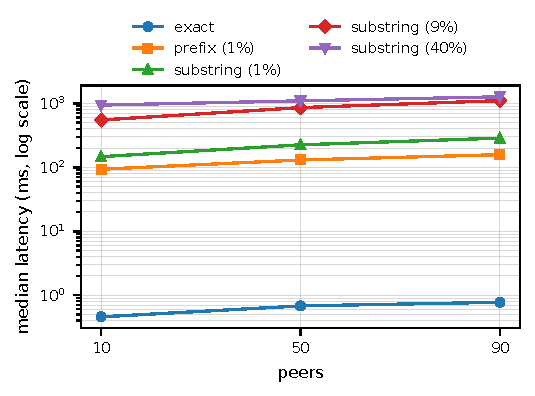
\includegraphics[width=\columnwidth]{figures/query_scaling.pdf}
\caption{Median query latency for 10,000 tuples and 16 index shards. Exact
reads stay below 1 ms; broad associative queries are dominated by index and
candidate work. The logarithmic axis is required to show both regimes.}
\label{fig:query-scaling}
\end{figure}

At 90 peers, the prefix, rare-substring, medium-substring, and common-substring
medians are 157, 286, 1,102, and 1,265 ms. Their 95th percentiles are 514, 647,
1,506, and 1,542 ms. More selective queries inspect fewer index nodes and
verify fewer candidates. The rare substring fetches a mean 608 PHT nodes;
the medium and common substrings fetch 1,868 and 2,046.

Logical traversal does not grow substantially with peer count for a fixed
catalog: the corresponding node counts at 10 peers are 599, 1,859, and 2,037.
The higher 90-peer latency therefore primarily reflects contention and
overlay/process overhead on the shared host, rather than an expanding search
tree. This distinction matters: the experiment demonstrates protocol behavior
under many peers but does not predict wide-area latency.

Catalog growth has a stronger effect on associative operations. At 90 peers,
increasing the catalog from 1,000 to 10,000 tuples raises the rare-substring
median from 123 to 286 ms and the common-substring median from 327 to
1,265 ms. The result follows from additional PHT traversal and candidate
verification, not from content transfer; query tuples remain small.

\subsection{The Shard Tradeoff}

Figure~\ref{fig:shards} separates the two sides of index sharding. Population
throughput rises from 26.2 tuples/s at one shard to 81.3 tuples/s at four, a
3.10$\times$ improvement, then falls to 72.1 tuples/s at 16. Sharding removes
one mutation bottleneck initially, but per-operation DHT work, scheduling, and
contention limit further gains on this host.

\begin{figure*}[t]
\centering
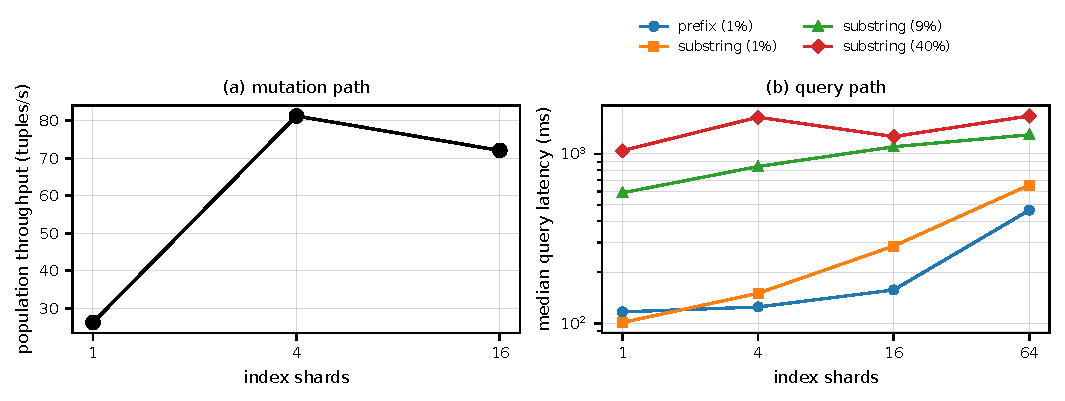
\includegraphics[width=0.94\textwidth]{figures/shard_tradeoff.pdf}
\caption{Index-shard tradeoff at 90 peers and 10,000 tuples. (a) Population
throughput compares only 1, 4, and 16 shards from one implementation revision.
(b) Every indexed query contacts the configured shards, so query latency tends
to rise with fanout; selectivity and host contention make the trend non-linear.}
\label{fig:shards}
\end{figure*}

Queries pay the other side. The rare-substring median rises from 101 ms with
one shard to 151, 286, and 655 ms with 4, 16, and 64 shards. The prefix query
rises from 117 to 465 ms across the same range. Broad queries are noisier
because candidate and host contention costs dominate fixed fanout: the
common-substring medians are 1,045, 1,646, 1,265, and 1,674 ms. Thus, shard
count should be chosen from measured mutation demand rather than maximized.

The 64-shard cell also reveals a useful degradation boundary. Associative
queries succeeded on an average of 62.5 of 64 shard reads; the prefix query
succeeded on 58. Nevertheless, all 600 associative trials in that cell reached
an exact owner and returned one verified match. Partial fanout can therefore
preserve \readop availability when a remaining shard contains a match, but it
does not provide complete enumeration and cannot prove absence. The API must
expose partial shard status to callers that need those stronger conclusions.

\subsection{Bloom Pruning}

Figure~\ref{fig:bloom} compares identical 90-peer, 10,000-tuple, 16-shard
queries with Bloom pruning on and off. For the rare substring, pruning reduces
median latency from 768 to 286 ms (2.69$\times$) and mean PHT nodes fetched
from 1,932 to 608 (3.18$\times$). Its 95\% median interval with pruning is
278--303 ms, versus 738--789 ms without it.

\begin{figure*}[t]
\centering
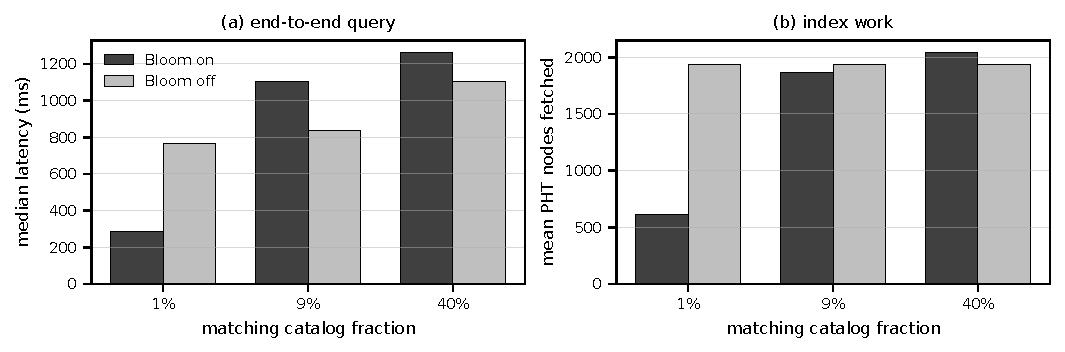
\includegraphics[width=0.94\textwidth]{figures/bloom_ablation.pdf}
\caption{Bloom ablation at 90 peers, 10,000 tuples, and 16 shards. Pruning is
valuable for the selective substring, but summary checking costs outweigh the
small amount of pruning for broad matches.}
\label{fig:bloom}
\end{figure*}

Bloom summaries are not uniformly beneficial. At 9\% selectivity they reduce
mean node fetches by only 3.3\% and increase median latency from 836 to
1,102 ms. At 40\%, pruning fetches more nodes in this workload and increases
the median from 1,106 to 1,265 ms. False-positive-safe verification preserves
correct returned matches, but summary reads and tests still cost time. A
production query planner should estimate selectivity and bypass Bloom traversal
for broad patterns rather than enable it indiscriminately.

\subsection{Concurrency and Failure Mechanisms}

Focused correctness tests complement the performance matrix. Concurrent
claim tests insert one tuple and race multiple \getop requests; the owner
returns one success and all other claimants observe absence or retry their
recorded result. Live-DHT handoff tests stop the exact owner after publication,
allow its lease to expire, and exercise a successor with a higher fence. The
three-peer test passed 20 of 20 repetitions without losing the committed tuple
or duplicating a consume. These tests validate the implementation mechanism
under the assumptions in Section~\ref{sec:semantics}; they are not evidence of
linearizable progress through arbitrary partitions.

A separate 100-peer mechanism case studies the storage path. The system
published an 8-MiB object to exactly seven providers, then stopped a proven
holder. A surviving provider served and hash-verified the object in 0.156 s.
Periodic repair restored seven providers in 51.281 s, retaining all six live
originals and admitting exactly one replacement. A cold non-provider then
fetched and verified it in 0.223 s. Across 24 observations, the provider count
stayed between six and seven and both end-to-end hashes passed. This is one
same-host trial: it validates bounded repair behavior, not a repair-time
distribution or regional-failure claim.

\subsection{Evaluation Summary}

The results support three conclusions. First, exact tuple ownership is cheap
relative to associative discovery and gives a clear place to enforce consuming
semantics. Second, sharding and Bloom summaries are workload-dependent tools:
four shards substantially improve insertion throughput, whereas 64 impose
large query fanout; Bloom pruning is excellent for selective negative
traversal but counterproductive for broad queries. Third, owner verification
lets reads degrade usefully under stale indexes or partial shard responses,
but successful lookup must not be confused with complete catalog enumeration.

\section{Related Work}
\label{sec:related}

\paragraph{Tuple spaces and coordination.}
Linda introduced generative communication through associative tuples and
separated coordination from the computation performed by participants
\cite{Gelernter1985,CarrieroGelernter1989}. Later systems adapted the model to
mobility and changing connectivity; LIME, for example, forms transient shared
tuple spaces among mobile components \cite{MurphyLIME}. \system shares the
indirect communication model but focuses on deterministic authority for
consuming operations, DHT-resident associative indexes, and references to a
content-addressed data plane. It is Linda-style, not a Linda deployment.

\paragraph{DHTs and distributed indexes.}
Kademlia routes exact keys through XOR distance with expected logarithmic
overlay hops \cite{MaymounkovKademlia}. PHT adds prefix and range lookup over a
DHT by distributing trie nodes \cite{RamabhadranPHT}. Bloom filters compactly
represent set membership with false positives but no false negatives for the
represented set \cite{Bloom1970}. \system combines these established
structures, then separates non-authoritative index discovery from
authoritative tuple execution. Its hash-sharded mutation owners address PHT
lost updates while making the resulting query-fanout cost explicit.

\paragraph{Content-addressed distributed storage.}
CFS distributes immutable blocks over Chord; OceanStore uses persistent
objects and untrusted infrastructure; Dynamo uses partitioning, replication,
and application-visible reconciliation for highly available key-value storage
\cite{DabekCFS,KubiatowiczOceanStore,DeCandiaDynamo}. IPFS combines
content-derived identifiers, Kademlia provider discovery, and peer-to-peer
block exchange \cite{Trautwein2022}. Bitswap and later IPFS work optimize
multi-provider content transfer \cite{deLaRochaBitswap}. Swarm and Filecoin
explore decentralized storage and, in Filecoin's case, incentive-backed
storage markets \cite{SwarmWhitepaper,FilecoinWhitepaper}. \system is not an
incentive or storage-market contribution. It adds an application-facing tuple
coordination plane and an explicit exclusive-consumption boundary to this
storage design space.

\paragraph{Consistency and replicated state.}
Dynamo's versioned, eventually reconciled values and CRDTs illustrate ways to
retain availability under concurrency without a single global order
\cite{DeCandiaDynamo,ShapiroCRDT}. \system uses version selection for DHT
records, but exclusive removal is not a commutative merge. It therefore routes
each exact name to one fenced serializer and sacrifices availability while
ownership is uncertain. This is a conscious consistency boundary rather than
a new general-purpose replication model.

\section{Limitations and Next Steps}
\label{sec:limitations}

The evaluation exposes several limitations that matter for a distributed
storage system.

First, exact-name safety across owner change depends on bounded clock error,
lease expiry, and convergence of DHT value selection. We have repeated
single-owner crash handoffs, but not multi-host partitions followed by
reconciliation. Until that test exists, \system should be described as fenced
crash recovery rather than partition-tolerant linearizability.

Second, mutations serialize at one elected owner per index shard. Four shards
improve population throughput in our workload, but 16 do not improve it
further, and indexed reads contact every shard. Authority should eventually be
adapted to load, and the query planner should stop early only when the caller
accepts non-exhaustive results. The 64-shard cell's partial responses reinforce
the need to distinguish ``one verified match'' from ``complete search.''

Third, index maintenance is eventually consistent. Owner verification prevents
stale positive entries from producing invalid reads or double consumes, but a
missing hint can hide a newly published name. Applications needing exhaustive
enumeration require an explicit completeness protocol or a consistency wait.
Bloom selection also needs a cost model because broad matches are slower with
pruning enabled.

Fourth, one 1-MiB record stores each exact-name multiset and retained request
results. Hot names and large queues need segmentation, and the bounded retry
window requires clients not to replay arbitrarily old request IDs. \system has
no multi-tuple transaction, compare-and-swap across names, POSIX namespace,
mutable byte ranges, or Byzantine metadata agreement.

Finally, the primary campaign runs many real peers and containers but only one
physical host. It measures implementation scaling, host contention, and
protocol work; it does not reproduce Internet latency, independent regional
failure, or correlated host loss. The 100-peer storage case is a single trial.
A multi-host campaign should therefore be the next evidence milestone, with
clock perturbation, partitions, regional provider loss, and repeated repair
distributions rather than one success case.

\section{Conclusion}

\system makes tuple-space coordination the center of a content-addressed
distributed store. Producers and consumers communicate through associative
tuples; exact owners serialize observation and exclusive claims; distributed
indexes find candidate names; and immutable content moves directly between
hash-verifying peers. ACAN uses the same tuple interface for active storage
metadata, while SMC2 selects currently available resources for placement and
repair.

The implementation and experiments show why the boundaries between these
roles matter. Exact-owner reads remain sub-millisecond at 90 same-host peers.
Index sharding improves insertion throughput but taxes every query. Bloom
summaries sharply reduce selective searches and slow broad ones. Authoritative
verification preserves a useful read result even when an index is stale or
partially reachable, but does not manufacture an exhaustive snapshot. Fenced
handoff and replica repair work under tested crash conditions without being
presented as consensus or regional resilience. These results position \system
as a concrete tuple-coordination substrate for decentralized workflows and
identify the consistency, query-planning, and multi-host evidence needed for
its next iteration.

% Balance the final page without adding a nonstandard package. IEEEtran moves
% reference 3 and later to the second column at this explicit trigger.
\IEEEtriggeratref{3}
\begin{thebibliography}{00}

\bibitem{Gelernter1985}
D. Gelernter, ``Generative communication in Linda,'' \emph{ACM Trans.
Program. Lang. Syst.}, vol. 7, no. 1, pp. 80--112, 1985.

\bibitem{CarrieroGelernter1989}
N. Carriero and D. Gelernter, ``Linda in context,'' \emph{Commun. ACM},
vol. 32, no. 4, pp. 444--458, 1989.

\bibitem{MurphyLIME}
A. L. Murphy, G. P. Picco, and G.-C. Roman, ``LIME: A middleware for
physical and logical mobility,'' in \emph{Proc. 21st Int. Conf. Distributed
Computing Systems}, 2001, pp. 524--533.

\bibitem{MaymounkovKademlia}
P. Maymounkov and D. Mazi\`eres, ``Kademlia: A peer-to-peer information
system based on the XOR metric,'' in \emph{Proc. IPTPS}, 2002, pp. 53--65.

\bibitem{RamabhadranPHT}
S. Ramabhadran, S. Ratnasamy, J. M. Hellerstein, and S. Shenker,
``Prefix Hash Tree: An indexing data structure over distributed hash
tables,'' in \emph{Proc. 23rd ACM Symp. Principles of Distributed Computing},
2004, pp. 368--377.

\bibitem{Bloom1970}
B. H. Bloom, ``Space/time trade-offs in hash coding with allowable
errors,'' \emph{Commun. ACM}, vol. 13, no. 7, pp. 422--426, 1970.

\bibitem{DabekCFS}
F. Dabek, M. F. Kaashoek, D. Karger, R. Morris, and I. Stoica,
``Wide-area cooperative storage with CFS,'' in \emph{Proc. 18th ACM Symp.
Operating Systems Principles}, 2001, pp. 202--215.

\bibitem{KubiatowiczOceanStore}
J. Kubiatowicz et al., ``OceanStore: An architecture for global-scale
persistent storage,'' in \emph{Proc. 9th Int. Conf. Architectural Support for
Programming Languages and Operating Systems}, 2000, pp. 190--201.

\bibitem{DeCandiaDynamo}
G. DeCandia et al., ``Dynamo: Amazon's highly available key-value store,''
in \emph{Proc. 21st ACM Symp. Operating Systems Principles}, 2007,
pp. 205--220.

\bibitem{Trautwein2022}
D. Trautwein et al., ``Design and evaluation of IPFS: A storage layer for
the decentralized web,'' in \emph{Proc. ACM SIGCOMM}, 2022, pp. 739--752.

\bibitem{deLaRochaBitswap}
A. de la Rocha, D. Dias, and Y. Psaras, ``Accelerating content routing with
Bitswap: A multi-path file transfer protocol in IPFS and Filecoin,'' in
\emph{Proc. IEEE Int. Conf. Blockchain and Cryptocurrency}, 2021, pp. 1--9.

\bibitem{SwarmWhitepaper}
V. Tr\'on et al., ``Swarm: Storage and communication infrastructure for a
self-sovereign digital society,'' Swarm Foundation, White Paper, 2021.

\bibitem{FilecoinWhitepaper}
J. Benet and N. Greco, ``Filecoin: A decentralized storage network,''
Protocol Labs, White Paper, 2017.

\bibitem{ShapiroCRDT}
M. Shapiro, N. Pregui\c{c}a, C. Baquero, and M. Zawirski,
``Conflict-free replicated data types,'' in \emph{Proc. 13th Int. Symp.
Stabilization, Safety, and Security of Distributed Systems}, 2011,
pp. 386--400.

\end{thebibliography}

\end{document}
